\chapter{สรุปผลการปฏิบัติงาน}
\label{chapter:experiment}

จากการสหกิจศึกษาเป็นเวลา 6 เดือน ตั้งแต่วันที่ \StartDWork ถึง \EndDWork ณ \Company

ในบทนี้ผู้เขียนได้สรุปกระบวนการดำเนินงานตั้งแต่เริ่มต้นโปรเจคไปจนจบโปรเจคที่ผู้เขียนได้เข้าไปมีส่วนร่วมในการทำงาน

นอกจากนี้ผู้เขียนได้สรุปรวบรวมและคัดสรรค์ช่องโหว่ที่พบเจอจากการค้นหาช่องโหว่ให้ลูกค้าของบริษัท และนำมาจัดกลุ่มตามหมวดหมู่ของ OWASP Top 10 ได้ดังนี้ โดยจะขอปิดชื่อบริษัทของลูกค้า และข้อมูลละเอียดอ่อนที่เป็นความลับของลูกค้า

\section{สรุปกระบวนการทำงาน}

\section{สรุปช่องโหว่ตามหวดหมู่ของ OWASP Top 10}

\subsection{Injection}

ในหัวข้อนี้จะพูดถึงการที่ผู้ประสงค์ร้ายสามารถแทรกคำสั่ง (Code) เข้าไปในระบบเพื่อให้ระบบทำงานตามที่ผู้ประสงค์ร้ายต้องการ พร้อมทั้งบอกถึงวิธีแก้ปัญหา

\subsubsection{SQL Injection}

เนื่องจากตัวเว็บแอปพลิเคชันรับ Input จากผู้ใช้ไปใช้งานโดยที่ไม่ได้ผ่านการตรวจสอบข้อมูล หรือทำความสะอาดข้อมูลก่อน ทำให้สามารถใส่คำสั่ง SQL เข้าไปทำงานได้ ความเสียหายจาก SQL Injection สามารถทำให้ผู้ประสงค์ร้ายเข้าถึงข้อมูลทุก ๆ อย่างที่อยู่ในฐานข้อมูลได้ด้วยสิทธิ์ของ Web Server หรือตามที่ผู้พัฒนาระบบกำหนดไว้ โดยระบบนี้เป็นระบบสำหรับค้นหาและเรียกดูข้อมูลย้อนหลังการทำธุรกรรม

\begin{figure}[h]
	\centering
	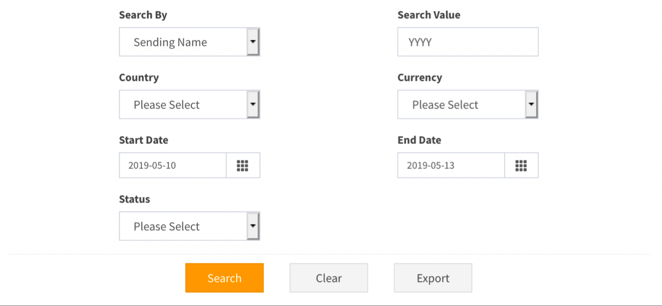
\includegraphics[width=0.8\columnwidth]{sqlisearchpage.png}
	\caption{หน้าค้นหาข้อมูล}
	\label{Fig:sqlisearchpage.png}
\end{figure}

เมื่อทดลองเรียกข้อมูลย้อนหลังตัว Browser จะส่ง Request ไปดังนี้

\begin{lstlisting}[numbers=none] 
POST [REDACTED]/dashboardV4.htm HTTP/1.1
[...]

cmd=getDashBoardTransaction&transactionType=OUW&searchBy=SENDING_NAME &searchValue=YYYY&currency=&country=&status=&startDate=2019-05-02&endDate=2019-05-13
\end{lstlisting}

ผู้ทดสอบใส่คำสั่ง SQL ดังต่อไปนี้ลงไปในค่าของตัวแปร searchBy

\begin{lstlisting}[language=sql,numbers=none] 
SENDING_NAME='YYYY' and '1'='1' and SENDING_NAME
\end{lstlisting}

จะได้ Request ดังต่อไปนี้

\begin{lstlisting}[numbers=none] 
POST [REDACTED]/dashboardV4.htm HTTP/1.1
[...]

cmd=getDashBoardTransaction&transactionType=OUW&<@\textcolor{red}{searchBy=SENDING\_NAME='YYYY' and '1'='1' and SENDING\_NAME}@>&searchValue=YYYY&currency=&country=&status=&startDate=2019-05-02&endDate=2019-05-13
\end{lstlisting}

เนื่องจากคำสิ่งที่เรา Inject เข้าไปนั้น จะมีค่าเป็น True เสมอ ซึ่งได้ Response ดังนี้ ซึ่งเป็น Response ที่มีข้อมูล

\begin{lstlisting}[numbers=none] 
HTTP/1.1 200 OK
Date: Mon, 13 May 2019 03:01:42 GMT
Content-Length: 3984
[...]

{"iTotalRecords":12,"iTotalDisplayRecords":12,"data":[[1,"1905101637LUZFN81","IRM","YYYY","George Adam1","567899000000","George Adam1","SGD","99.02","THB","37.58","31.3200000","FA","318013"]]
[...]
\end{lstlisting}

จากนั้นทดสอบใส่คำสั่ง SQL ดังต่อไปนี้ลงไปในค่าของตัวแปร searchBy แต่ครั้งนี้คำสั่งที่ใส่ไปจะมีค่าเป็น False

\begin{lstlisting}[language=sql,numbers=none] 
SENDING_NAME='YYYY' and '1'='0' and SENDING_NAME
\end{lstlisting}

จะได้ Request ดังต่อไปนี้

\begin{lstlisting}[numbers=none] 
POST [REDACTED]/dashboardV4.htm HTTP/1.1
[...]

cmd=getDashBoardTransaction&transactionType=OUW&<@\textcolor{red}{searchBy=SENDING\_NAME='YYYY' and '1'='0' and SENDING\_NAME}@>&searchValue=YYYY&currency=&country=&status=&startDate=2019-05-02&endDate=2019-05-13
\end{lstlisting}

Response ที่ได้กลับมาไม่มีข้อมูลอะไรอยู่เลย

\begin{lstlisting}[numbers=none] 
HTTP/1.1 200 OK
Date: Mon, 13 May 2019 03:01:42 GMT
Content-Length: 54
[...]

{"iTotalRecords":0,"iTotalDisplayRecords":0,"data":[]}
\end{lstlisting}

ดังนั้นจึงยืนยันได้ว่าคำสั่ง SQL ที่ใส่เข้าไปถูกตัวเว็บแอปพลิเคชันนำไปทำงาน ซึ่งตัวแปรที่ทำให้เกิดช่องโหว่นี้คือตัวแปร searchBy

วิธีการแก้ไขคือควรใช้ SQL Prepare Statements แทนการเชื่อม String เนื่องจากส่วนข้อมูล Input กับ คำสั่งจะไม่ถูกนำมาต่อกันโดยตรง ถ้าไม่สามารถใช้ SQL Prepare Statement ได้ เนื่องจากข้อจำกับของภาษา หรือ Framework ก็ไม่ควรนำ Input จาก User เข้าไปใช้กับ Database โดยตรง

ซึ่งหมายความว่าตัวอักขระพิเศษเช่น Single Quote (') หรือ Double Quote (") จะต้องถูก Escape ก่อน (แปลงจาก ' เป็น \') เพื่อให้ Database มองว่าเป็นข้อมูล ไม่ใช่คำสั่ง

นอกจากนี้ยังควรกรองข้อมูล Input ด้วยวิธีแบบ Whitelist เช่นเลข ID สินค้าควรเช็คที่ฝั่ง Server ว่าประกอบไปด้วยตัวเลขเท่านั้น เป็นต้น และควรกรอกข้อมูลกับทุก ๆ Input ที่ผู้ใช้สามารถใส่เข้ามาได้ เช่น Cookie, Form ที่ถูกซ่อนอยู่ และ Request Header ต่าง ๆ เป็นต้น

แต่ทว่าในกรณีนี้ SQL Prepare Statement ไม่สามารถใช้ได้กับข้อมูลที่เป็น Metadata ของ Database เช่น ชื่อ Table, Column เป็นต้น ดังนั้นควรใช้กระบวนการกรองข้อมูลแบบ Whitelist กล่าวคือมี List ของชื่อ Column ที่ใช้ได้ หากข้อมูลที่ได้รับมาอยู่นอกเหนือจาก List ที่มีให้ปฏิเสธข้อมูลนี้ทันที

\subsubsection{Broken Authentication}

\subsubsection{Sensitive Data Exposure}

\subsection{XML External Entities (XXE)}

\subsection{Broken Access Control}

\subsubsection{Security Misconfiguration}

\subsubsection{Cross-Site Scripting}

\subsubsection{Insecure Deserialization}

\subsubsection{Using Components with Known Vulnerabilities}

\subsubsection{Insufficient Logging and Monitoring}

Log เปรียบเสมือนสมุดบันทึกประจำวันของคนเรา ไม่ว่าจะเกิดเหตุการณ์อะไรขึ้น เราก็จะจดบันทึกเหตุการณ์นั้น ๆ ลงในสมุดบันทึก ในทางคอมพิวเตอร์ก็เช่นกัน ตั้งแต่เปิดเครื่อง จนปิดเครื่อง หรือเปิดโปรแกรม จนปิดโปรแกรมก็ต้องเกิดเหตุการณ์ต่าง ๆ มากมาย ซึ่งคอมพิวเตอร์จะบันทึกเหตุการณ์ต่าง ๆ ไว้ในไฟล์ (Log File)

ตัวอย่างข้อมูลไฟล์บันทึกเหตุการณ์ของ Web Application ที่เขียนด้วย Spring Boot

\begin{figure}[h]
	\centering
	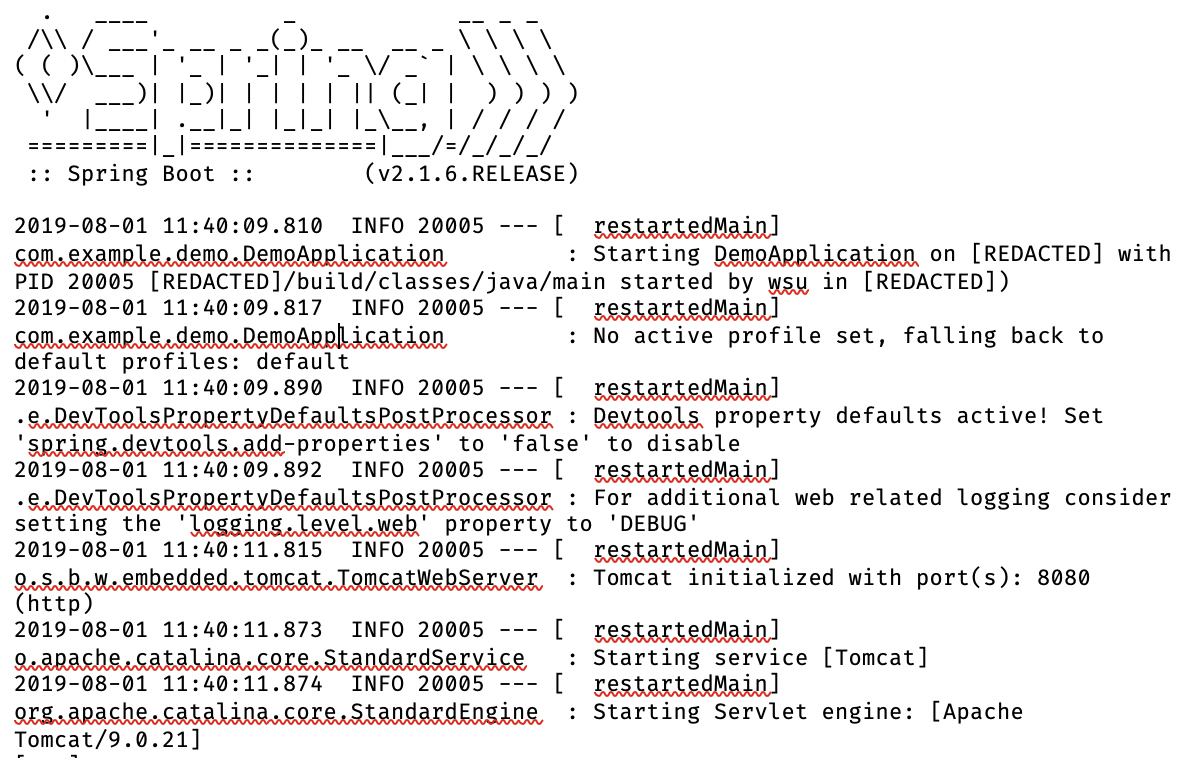
\includegraphics[width=0.8\columnwidth]{springbootlog.png}
	\caption{ตัวอย่าง Log ของ Spring Boot Web Framework}
	\label{Fig:springbootlog.png}
\end{figure}

แต่ละบรรทัดจะบ่งบอกถึงเหตุการณ์ต่าง ๆ เช่น ใช้ไฟล์ตั้งค่าไฟล์ไหน โปรไฟล์อะไร เปิด Port อะไรอยู่ เป็นต้น

และถ้าหากระบบสารสนเทศเราประกอบไปด้วยหลาย ๆ ส่วน เช่น Spring Boot สำหรับส่วนเว็บแอปพลิเคชัน PostgreSQL สำหรับฐานข้อมูล Redis สำหรับเก็บ Session ของผู้ใช้งาน เป็นต้น นั่นหมายความว่าหากเกิดข้อผิดพลาดในระบบ ก็ต้องไล่เปิดไฟล์ทีละไฟล์เพื่อหาสาเหตุ ซึ่งเป็นการกระทำที่ช้า แต่ทว่าในบางบริษัทที่ผู้เขียนไปทำ Penetration Testing ยังคงใช้วิธีการข้างต้นอยู่ ทำให้เมื่อมีเหตุการณ์อะไรเกิดขึ้น กว่าจะค้นหาต้นตอได้ก็จะกินเวลานานมาก

ดังนั้นหากต้องการจัดการกับข้อมูล Log อย่างมีประสิทธิ์ภาพควรใช้ Tools เข้ามาช่วยจัดการ Log เครื่องมือที่นิยมในปัจจุบันคือ ELK Stack ซึ่งประกอบไปด้วย Elasticsearch\cite{}, Logstash\cite{} และ Kibana\cite{}

สมมุติว่าเกิดเหตุการณ์ Brute Force Directory ขึ้นมาบนเว็บแอปพลิเคชัน เราสามารถค้นหาได้ทันทีว่าเกิดการ Brute Force ตั้งแต่เวลาใดถึงเวลาใด แล้วผู้กระทำได้ Brute Force Directory อะไรไปแล้วบ้าง

\begin{figure}[h!]
	\centering
	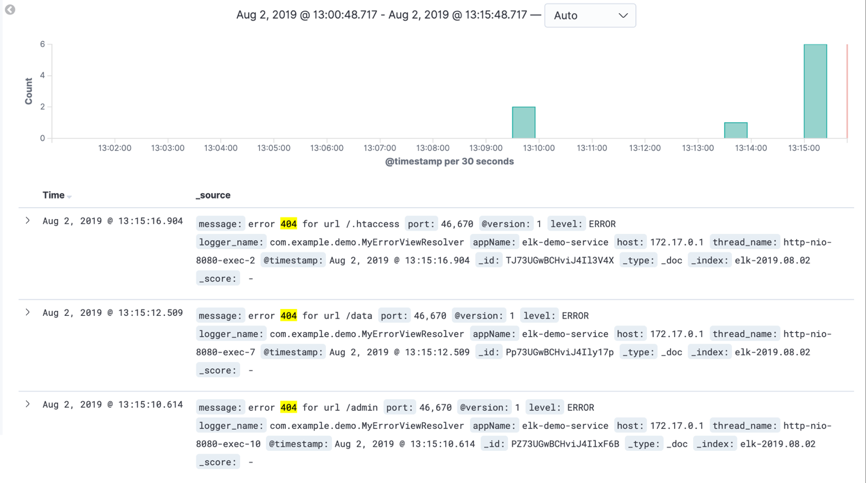
\includegraphics[width=0.8\columnwidth]{404errorlog.png}
	\caption{ผลลัพธ์เมื่อค้นหา Error 404 ในช่วงเวลา 15 นาทีที่ผ่านมา}
	\label{Fig:404errorlog.png}
\end{figure}
